\section{Navigation}\label{sec:navigation}

The internal computer of the GVR-Bot passes sensor data to the on-board, external embedded computer for processing, map generation, and development of a navigation scheme. The external embedded computer is directly connected and receives updates from the LIDAR in real-time. The tilting capability of the LIDAR allows 3-D point cloud data to be collected for use in developing a 3-D navigation solution. For ARIBO-IH missions, accurate inertial measurements are not required because navigation occurs in highly structured indoor environments, and odometry data helps mitigate errors in position. The computer then uses the laser data to generate a 2-D planar occupancy grid map. The technique of using occupancy grid maps based on LIDAR scans is being implemented because it can be done at a low cost computationally, and it is a proven approach for localizing a ground robot in a real-world setting \cite{thrun2005probabilistic,kohlbrecher2011flexible}. The 2-D SLAM information is coupled with a 3-D pose estimate that is generated using an Extended Kalman Filter (EKF). This coupling allows the 2-D planar map to be overlayed with robot pose data estimated via EKF. 

This information is locally stored in memory for purposes of future unplanned events that may occur during the mission, such as connection loss. The highly detailed 3-D map and a 2-D planar map are generated, while a coarser version of the 2-D map is created for the purposes of wireless transmission to the control unit to be displayed on the GUI for the user. This multi-resolution map representation does not rely on any type of filtering or downsampling, but it simultaneously generates multiple maps of different resolutions that have scalability and low cost computationally. This approach is further described in \cite{kohlbrecher2011flexible,habbecke2006iterative}. The high computation capability of the computer allows for both the SLAM and 3-D EKF components to be run at soft real-time with a low enough latency in calculation that it is negligible compared to actual or hard real-time 3-D navigation schemes.

\subsection{Practical Implementation}\label{sec:practical}

The Stanford Linear Accelerator Center (SLAC) National Accelerator Laboratory has partnered with TARDEC and West Point to field a GVR-Bot for use in the two-mile long tunnel. Currently, maintenance crews must traverse the tunnel and visually inspect for gases, liquids, radiation, vibrations, ultrasonic frequencies, and atmospheric effects that could be harmful to humans. As previously described, the GVR-Bot navigates the tunnel as shown in Fig.~\ref{fig:tunnel} which is generally clear of debris and has known features throughout the corridor. Sensor packages are installed as described in Sec. \ref{sec:sensors} and the graphical interface provides robot pose and environmental information as discussed in Sec. \ref{sec:ui}.

\begin{figure}
	\centering
	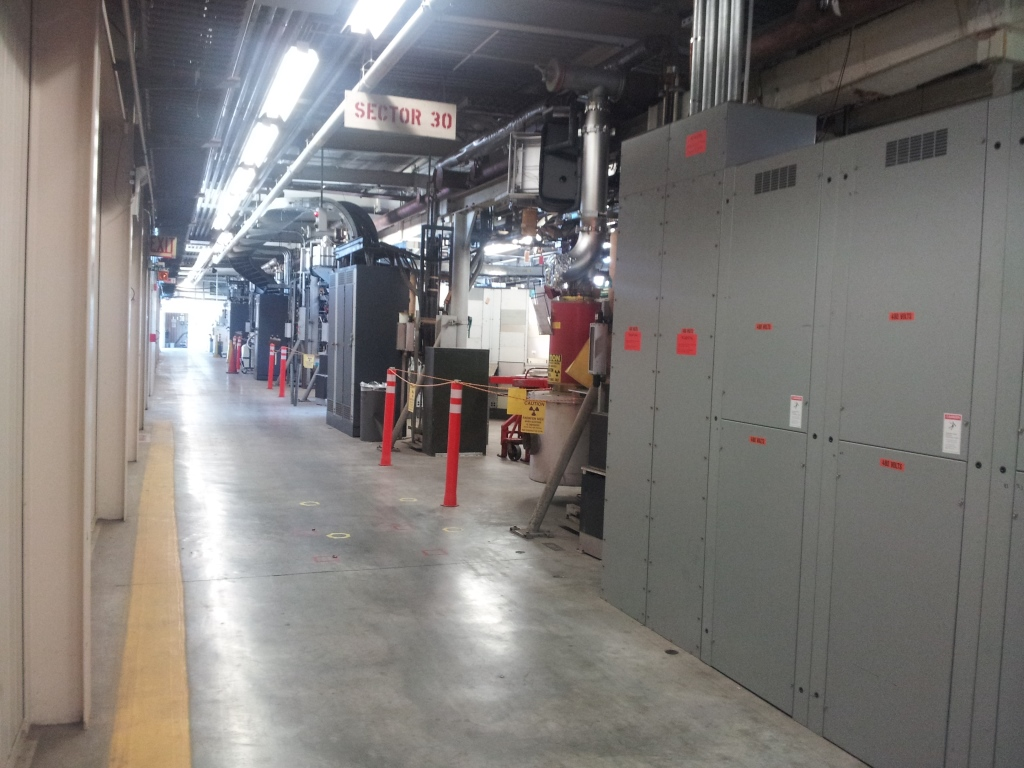
\includegraphics[width=0.48\textwidth]{./pictures/slac-tunnel.jpg}
	\caption{Interior corridor of SLAC tunnel.}
	\label{fig:tunnel}
\end{figure}
